% Chapter Template

\chapter{Diseño e Implementación} % Main chapter title

\label{Chapter3} % Change X to a consecutive number; for referencing this chapter elsewhere, use \ref{ChapterX}
En el siguiente capítulo se presenta el diseño y la implementación de las tres partes fundamentales del equipo. Se abarcan aspectos de diseño de hardware, desarrollo de firmware, diseño y fabricación mecánica.
%----------------------------------------------------------------------------------------
%	SECTION 1
%----------------------------------------------------------------------------------------

\definecolor{mygreen}{rgb}{0,0.6,0}
\definecolor{mygray}{rgb}{0.5,0.5,0.5}
\definecolor{mymauve}{rgb}{0.58,0,0.82}
%%%%%%%%%%%%%%%%%%%%%%%%%%%%%%%%%%%%%%%%%%%%%%%%%%%%%%%%%%%%%%%%%%%%%%%%%%%%%
% parámetros para configurar el formato del código en los entornos lstlisting
%%%%%%%%%%%%%%%%%%%%%%%%%%%%%%%%%%%%%%%%%%%%%%%%%%%%%%%%%%%%%%%%%%%%%%%%%%%%%
\lstset{ %
  backgroundcolor=\color{white},   % choose the background color; you must add \usepackage{color} or \usepackage{xcolor}
  basicstyle=\footnotesize,        % the size of the fonts that are used for the code
  breakatwhitespace=false,         % sets if automatic breaks should only happen at whitespace
  breaklines=true,                 % sets automatic line breaking
  captionpos=b,                    % sets the caption-position to bottom
  commentstyle=\color{mygreen},    % comment style
  deletekeywords={...},            % if you want to delete keywords from the given language
  %escapeinside={\%*}{*)},          % if you want to add LaTeX within your code
  %extendedchars=true,              % lets you use non-ASCII characters; for 8-bits encodings only, does not work with UTF-8
  %frame=single,	                % adds a frame around the code
  keepspaces=true,                 % keeps spaces in text, useful for keeping indentation of code (possibly needs columns=flexible)
  keywordstyle=\color{blue},       % keyword style
  language=[ANSI]C,                % the language of the code
  %otherkeywords={*,...},           % if you want to add more keywords to the set
  numbers=left,                    % where to put the line-numbers; possible values are (none, left, right)
  numbersep=5pt,                   % how far the line-numbers are from the code
  numberstyle=\tiny\color{mygray}, % the style that is used for the line-numbers
  rulecolor=\color{black},         % if not set, the frame-color may be changed on line-breaks within not-black text (e.g. comments (green here))
  showspaces=false,                % show spaces everywhere adding particular underscores; it overrides 'showstringspaces'
  showstringspaces=false,          % underline spaces within strings only
  showtabs=false,                  % show tabs within strings adding particular underscores
  stepnumber=1,                    % the step between two line-numbers. If it's 1, each line will be numbered
  stringstyle=\color{mymauve},     % string literal style
  tabsize=2,	                   % sets default tabsize to 2 spaces
  title=\lstname,                  % show the filename of files included with \lstinputlisting; also try caption instead of title
  morecomment=[s]{/*}{*/}
}

\section{Hardware}
\subsection{Diseño basado en módulos de hardware libre}
\label{subsection:Diseño basado en módulos de hardware libre}

Para la implementación del hardware se utilizó el software libre de diseño de circuitos impresos KICAD \citep{web_kicad}, la elección del mismo se basó en que sus últimas versiones presentaron mejoras significativas respecto a sus predecesoras.

El diseño de la placa electrónica se baso en el estudio de los siguientes módulos:
\begin{itemize}
\item TMC5130-EVAL \citep{3_web_trinamic_placa}	
\item NodeMCU \citep{web_nodemcu}
\end{itemize}
Se destaca que ambos proyectos adhieren a la filosofía del hardware libre. Por lo tanto se pudieron descargar y estudiar los diagramas esquemáticos de ambas placas. 

El módulo TMC5130-EVAL, como se describió en la sección \ref{sec:Circuitos integrados Trinamic}, contiene al CI TMC5130. Del estudio de esta placa de evaluación se extrajeron las configuraciones necesarias para lograr la correcta utilización del driver. Se tuvieron en cuenta las recomendaciones de diseño establecidas por el fabricante, como por ejemplo: la incorporación de un clock externo de 16 MHz como se observa en la figura \ref{fig:kicad_clock} el cual es necesario en aplicaciones de alta precisión. 

\begin{figure}[h]
	\centering
	\includegraphics[width=.5\textwidth]{./Figures/kicad_clock.png}
	\caption{Clock para el CI TMC5130.}
	\label{fig:kicad_clock}
\end{figure}

Otra etapa importante, como se observa en la figura \ref{fig:kicad_tension}, es el regulador de tensión que permite alimentar al equipo con tensiones continuas de entre 24 V y 46 V. Para dicho fin se utilizo el CI LM5161 en su configuración \textit{step-down buck converter}. 
El equipo fue diseñado para ser alimentado con una fuente externa de tensión continua, simplificando así cuestiones regulatorias de certificación que deben cumplir equipos que se alimentan directamente a la red eléctrica.


\begin{figure}[h]
	\centering
	\includegraphics[width=1\textwidth]{./Figures/kicad_tension.png}
	\caption{Módulo de entrada.}
	\label{fig:kicad_tension}
\end{figure}
 
A continuación se observan en la figura \ref{fig:kicad_trinamic} las conexiones del driver con el motor paso a paso y el puerto SPI utilizado para la comunicación con el microcontrolador. 
 
\begin{figure}[h]
	\centering
	\includegraphics[width=1\textwidth]{./Figures/kicad_trinamic.png}
	\caption{CI TMC5130.}
	\label{fig:kicad_trinamic}
\end{figure} 
 
El módulo NodeMCU es una placa de desarrollo que contiene el SoC ESP32-WROOM. A partir del estudio de su diseño, se implementó la etapa conversora SERIAL-USB que puede observase en la figura \ref{fig:kicad_conversor}. El mismo permite conectar el módulo directamente a un puerto USB de computadora para descargar el firmware y establecer una comunicación a través del periférico UART. Esto evita tener que contar con un programador externo para comunicarse con el equipo.
\begin{figure}[h]
	\centering
	\includegraphics[width=1\textwidth]{./Figures/kicad_conversor.png}
	\caption{Conversor UART-USB.}
	\label{fig:kicad_conversor}
\end{figure}

%\begin{figure}[h]
%	\centering
%	\includegraphics[width=.6\textwidth]{./Figures/kicad_esp.png}
%	\caption{Módulo ESP32.}
%	\label{fig:kicad_esp}
%\end{figure}
  
Finalmente, se observa en la figura \ref{fig:dip_3d_model} el diseño 3D generado por el software KICAD. El mismo se encuentra disponible en los repositorios de la empresa TECSCI \citep{web_hardware_tecsci}. La placa electrónica de este equipo dip coater cuenta con licencia CERN OHL v.1.2 \citep{web_cern_licence}.


\begin{figure}[h]
	\centering
	\includegraphics[width=.5\textwidth]{./Figures/dip_3d_model.pdf}
	\caption{Modelo 3D Kicad.}
	\label{fig:dip_3d_model}
\end{figure}
         



  
%-----------------------------------
%	SUBSECTION 1
%-----------------------------------
\subsection{Fabricación}
%-----------------------------------
%	SUBSECTION 2
%-----------------------------------
La placa electrónica se fabricó con el proveedor local de circuitos impresos Ernesto Mayer S.A. \citep{web_mayer}. A continuación se presenta la información de diseño de la placa y se describen algunas  restricciones de diseños impuestas por el fabricante:

\begin{itemize}

\item Grilla de posicionamiento principal: 0.25 mm
\item Grilla de ruteo principal: 0.25 mm
\item Agujeros de montaje: 3.2 mm
\item Pistas principales: 0.5 mm
\item Pistas inferiores: 0.25 mm (límite particular 8 mils(0.20mm))
\item Pistas superiores: 0.8 mm
\item Vías: 0.8 mm /0.4 mm (límite particular 8 mils(0.20mm))
\item Margen general: 0.22 mm
\item Margen particular: 0.2 mm (límite particual 8 mils(0.20 mm))
\item Fabricación: espesor 1.6mm FR4  
\item Restricciones generales del fabricante: estándar 10 mils( 0.254 mm)

\end{itemize}

Luego de fabricar el PCB, se continuó con el montaje de componentes electrónicos superficiales, que estuvo a cargo de la empresa Asembli S.A. \citep{web_asembli}. Se fabricó un primer lote de cinco placas.


\begin{figure}[htbp]
	\centering
	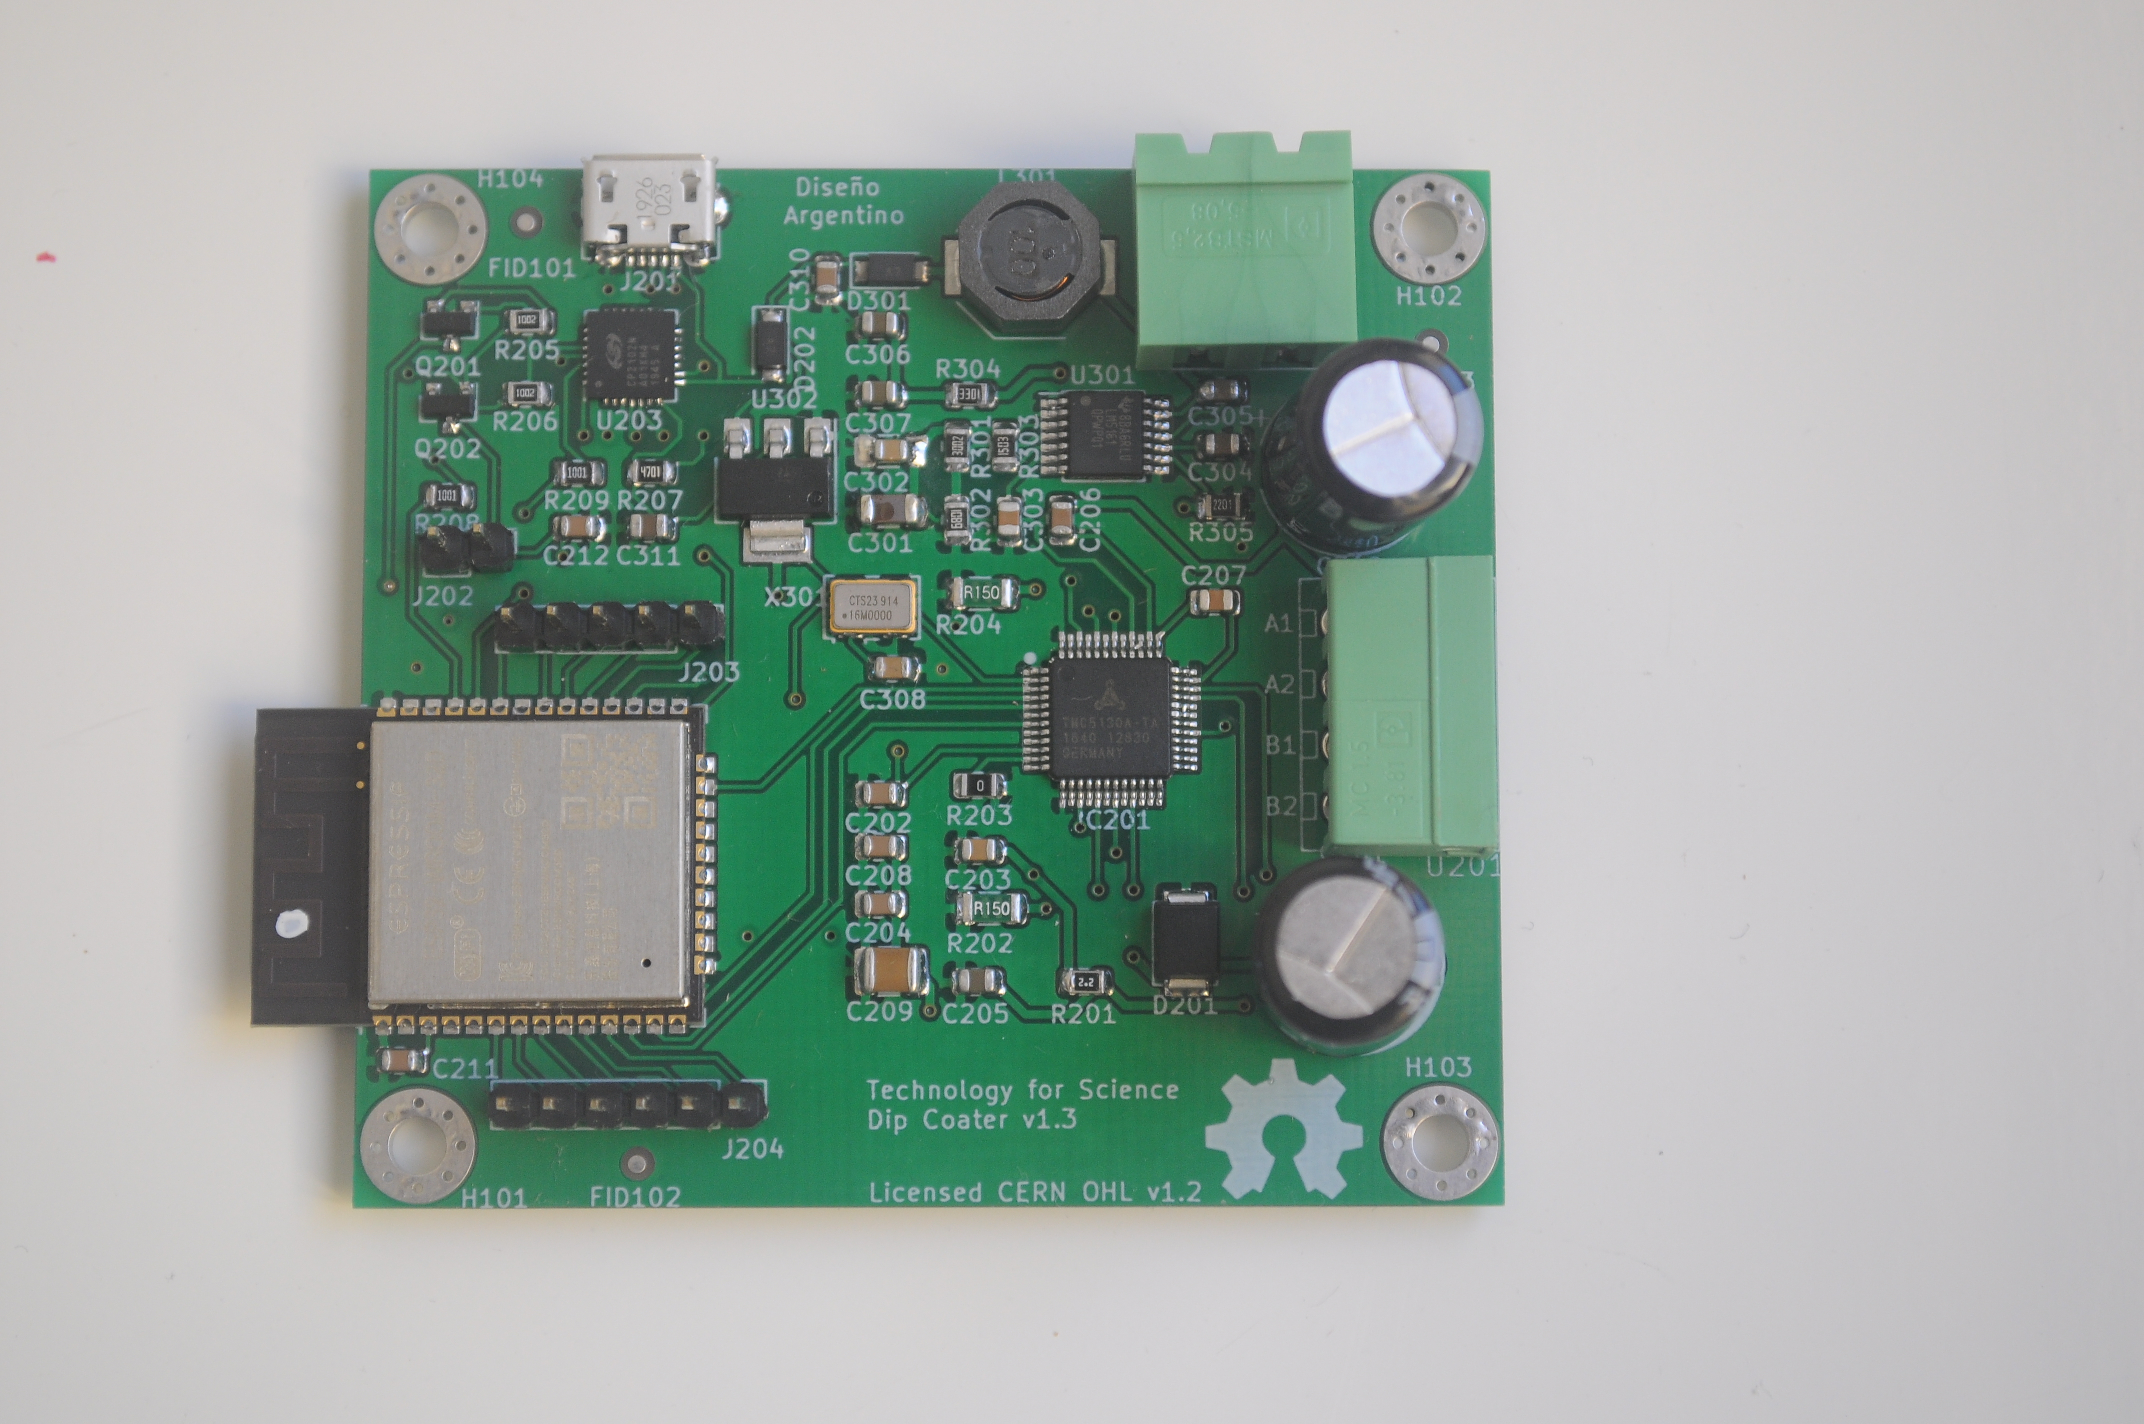
\includegraphics[width=1\textwidth]{./Figures/dip_real_model.png}
	\caption{Placa fabricada MAYER SRL.}
	\label{fig:dip_real_model}
\end{figure}

%----------------------------------------------------------------------------------------
%	SECTION 2
%----------------------------------------------------------------------------------------

\section{Firmware}
\subsection{Capas de abstracción}

Para la implementación del firmware se trabajó con el \textit{framework} ESP-IDF \citep{web_esp_idf} provisto por el fabricante del microcontrolador. Dicho entorno se ejecuta sobre FreeRTOS, que es un sistema operativo de tiempo real utilizado en dispositivos embebidos que permite un desarrollo de software bajo un esquema multi-tareas.

Se desarrolló un firmware modular que atomiza el funcionamiento en diferentes bloques de software, lo cual permite incorporar código de manera incremental y ordenada. Se observan en la figura \ref{fig:capas} las capas de abstracción de software implementadas.

La idea principal de esta modularización es la de no permitir llamados a funciones entre capas discontinuas. Los módulos de la capa superior o capa APP solo pueden hacer llamados a funciones de la capa intermedia o capa API \textit{(Application Programming Interfaces)} y estos últimos solo pueden llamar a funciones de la capa inferior o capa BOARD.


\begin{figure}[h]
	\centering
	\includegraphics[width=1\textwidth]{./Figures/capas.jpg}
	\caption{Capas de abstracción de software.}
	\label{fig:capas}
\end{figure}


La capa tres corresponde a la capa de aplicaciones. El firmware cuenta con 3 aplicaciones fundamentales para el funcionamiento del equipo y una aplicación de testing utilizada para probar nuevos componentes de software. Cada aplicación contiene al menos una \textit{task} del sistema operativo freeRTOS.

\begin{itemize}

\item APP coating: se encarga de la comunicación con el driver TMC5130 y de la ejecución de todos los movimientos.
\item APP consola: administra una consola de comandos que permite ejecutar y configurar el equipo a través de una comunicación serial, recibe comandos en la consola serial y los envía a traves de una cola de freeRTOS a la app coating para ser procesados.
\item APP hmi: administra la interfaz de configuración, establece una comunicación serial con la pantalla táctil, recibe comandos a través de una cola de freeRTOS y los envía a la app coating para ser procesados.
\item APP test: se utiliza para probar nuevos componentes y realizar tests sobre el sistema. Se activa y desactiva según la necesidad de uso.

\end{itemize}
% y realizar test sobre el sistema que se activa y desactiva según la necesidad de uso.

La capa dos esta compuesta por bloques de código provistos por los fabricantes de drivers.
\begin{itemize}
\item API TMC: provista por el fabricante Trinamic y adaptada para ser ejecutada bajo el framework ESP-IDF.
\item API BOSH: provista por el fabricante y adaptada a este firmware.
\item API TECSCI: contiene los módulos de software para el manejo de la capa BOARD, es un módulo que está en constante crecimiento con los diferentes desarrollos que la compañia TECSCI va ejecutando.
\end{itemize}

La capa uno interacciona con los módulos de hardware del microcontrolador, es decir, que esta capa es la única que contiene todos los llamados a funciones disponibles en el framework ESP-IDF, llamados a periféricos como por ejemplo: UART, GPIO, SPI, I2C entre otros, son realizados desde esta capa. En el caso de que en un futuro se quiera realizar un cambio de microcontrolador, esta sería la única capa que debería reescribirse en mayor medida, permitiendo así reutilizar el software escrito en capas superiores.

Cabe aclarar que este diseño de software es un concepto que se fue implementando a través de las sucesivas refactorizaciones del firmware actual y es posible entonces encontrar algunas excepciones de diseño. Las mismas se irán corrigiendo en futuras actualizaciones.


\subsection{Módulos principales de software}
\label{sec:modulos principales}
\subsubsection{Control de movimientos}

La aplicación app coating contiene toda la lógica de control de movimientos, la misma se encarga de realizar toda la configuración inicial del driver TMC5130, de ejecutar los procesos completos de dip coating y de procesar comandos individuales para generar diferentes tipos de movimientos. 

Como se mencionó en la subsección \ref{subsection:Driver TMC5130} la configuración inicial del driver es compleja, por tal motivo se utilizo el software  TMCL-IDE provisto por el fabricante para realizar una configuración interactiva de todos los registros internos del driver. Cabe destacar que con este software se pueden configurar todos los driver que la compañía ofrece, abarcando desde motores paso a paso hasta  servomotores, motores \textit{brushless} y de corriente continua. 

En esta etapa de configuración es recomendable que el motor este acoplado al eje lineal, junto con el tornillo, la tuerca y el carro ya que el driver registra la corriente que circula por las bobinas del motor y calcula la fuerza contraelectromotriz que el eje esta ejerciendo. 
En la siguiente figura \ref{fig:tmcl_ide} se observa el entorno de desarrollo TMCL-IDE.  

\begin{figure}[h!t]
	\centering
	\includegraphics[width=1\textwidth]{./Figures/tmcl_ide_1.png}
	\caption{Software TMCL-IDE.}
	\label{fig:tmcl_ide}
\end{figure}


A continuación en la figura \ref{fig:tmcl_ide_stall} se puede observar el \textit{wizard} de configuración de las funciones \textit{stallguard2} y \textit{coolstep}.
Como se mencionó en el capítulo \ref{Chapter2} es posible usar stallguard2 para detectar un limite mecánico de recorrido o final de carreta, el parámetro \textit{stall guard threshold} relaciona la fuerza contraelectromotriz que el driver registra, a medida que mayor fuerza es detectada, es decir mayor corriente en los motores, el valor de stallguard2 disminuye. Se debe entonces configurar un valor de detección para que el driver pueda generar un aviso.
El firmware cuenta con una funcion llamada \textit{mod-coating-process-cero-machine} que se encarga de detectar la señal que el driver enviá cuando se detecta un final de carrera. La misma se encarga de parar el motor, generar un desplazamiento en sentido contrario y establecer la nueva posición.

  

\begin{figure}[h!t]
	\centering
	\includegraphics[width=1\textwidth]{./Figures/tmcl_ide_2.png}
	\caption{Configuración de funcionalidades stalldguard2 y coolstep.}
	\label{fig:tmcl_ide_stall}
\end{figure}

Otros parámetros importantes a configurar son los que definen la rampa de aceleración del desplazamiento. 
Como se observa en la figura \ref{fig:rampa} es posible definir dos aceleraciones y dos desaceleraciones hasta llegar a una velocidad deseada.  
\begin{figure}[h!]
	\centering
	\includegraphics[width=1\textwidth]{./Figures/rampa_1.png}
	\caption{Configuración de rampa de seis puntos.}
	\label{fig:rampa}
\end{figure}

Todos los movimientos del equipo dip coater están definidos de la siguiente manera.
\begin{lstlisting}[label=cod:vControl,caption=Macros para configurar de desplazamientos.] 
	// Velocidad
	//V1
	Evalboards.ch1.writeRegister(0, TMC5130_V1, (arg->velocity) / 2);
	//VMAX
	Evalboards.ch1.writeRegister(0, TMC5130_VMAX, arg->velocity);
	//VSTART
	Evalboards.ch1.writeRegister(0, TMC5130_VSTART, 0);
	//VSTOT
	Evalboards.ch1.writeRegister(0, TMC5130_VSTOP, 100);

	// Seteo Aceleracion
	//A1
	Evalboards.ch1.writeRegister(0, TMC5130_A1,  arg->acceleration);
	//AMAX
	Evalboards.ch1.writeRegister(0, TMC5130_AMAX,  arg->acceleration);

	// Seteo Desaceleracion

	//DMAX
	Evalboards.ch1.writeRegister(0, TMC5130_DMAX,  arg->acceleration);
	//D1
	Evalboards.ch1.writeRegister(0, TMC5130_D1,  arg->acceleration);
\end{lstlisting}

Es decir que se genera una rampa de cuatro puntos al establecer las siguientes relaciones de variables:
\begin{itemize}
\item A1 = AMAX  (Aceleración establecida por usuario).
\item D1 = DMAX  (Desaceleración establecida por usuario).
\item VMAX 	  (Velocidad establecida por usuario).
\item V1 = VMAX / 2 (Velocidad fija del movimiento).

\end{itemize}


 

App coating puede recibir a través de implementaciones de colas de FreeRTOS comandos de ejecución desde la app hmi y desde app consola.

\subsubsection{Interfaz usuario-máquina}
Las aplicaciones app consola y app hmi se encargan de la comunicación con el usuario del equipo.
 
App consola permite establecer un canal de comunicación entre el equipo dip coater y un ordenador a través de una comunicación UART. Como se mencionó en la subsección \ref{subsection:Diseño basado en módulos de hardware libre} la placa electrónica incorpora un conversor UART-USB que permite conectar los equipos directamente a través de un cable USB. Se observan a continuación los comandos definidos en la consola para poder interactuar con el equipo.

\begin{figure}[h!]
	\centering
	\includegraphics[width=1\textwidth]{./Figures/consola_2.png}
	\caption{Comandos de movimientos.}
	\label{fig:consola_movimientos}
\end{figure}

Y por último como se observa en la figura \ref{fig:consola_comandos} comandos que sirven para leer o escribir registros del driver y para consultar información del sistema.
\begin{figure}[h!]
	\centering
	\includegraphics[width=0.7\textwidth]{./Figures/consola_3.png}
	\caption{Comandos de control.}
	\label{fig:consola_comandos}
\end{figure}

Como ejemplo se observa a continuación en la figura \ref{fig:comando_lectura} una consulta al registro XACTUAL (0x21) que contiene la posición expresada en micro pasos desde la referencia inicial donde esta posicionado el carro , y luego una consulta al registro XTARGET (0x2D), que en este caso como el carro se encuentra detenido coinciden en valor. XTARGET es uno de los registros que debe modificarse cuando se desea realizar un movimiento. El valor hace referencia a la posición objetivo que se desee llegar establecida en micro pasos.

\begin{figure}[h!]
	\centering
	\includegraphics[width=1\textwidth]{./Figures/consola_6.png}
	\caption{Comandos de lectura sobre el driver TMC5130.}
	\label{fig:comando_lectura}
\end{figure}


Cada vez que el usuario acciona un comando de movimiento o de control del proceso dip coating se envía la orden a través de una cola de FreeRTOS hacia la app coating que se encarga de procesar y ejecutar dicho comando.

Si la maquina esta ejecutado un movimiento individual o un proceso dip coating completo y se le enviá un comando, el mismo por seguridad y para evitar que se encolen los movimientos es descartado . En la figura 
\ref{fig:consola_comando_ok} se observa que luego de iniciado el proceso dip coating se envia el comando DOWN y el mismo es descartado sin afectar el proceso.

\begin{figure}[h!]
	\centering
	\includegraphics[width=1\textwidth]{./Figures/consola_4.png}
	\caption{Comandos de lectura sobre el driver TMC5130.}
	\label{fig:consola_comando_ok}
\end{figure}

El único comando de movimiento que no es descartado es el comando STOP, por seguridad este es el único  comando con tratamiento especial y en cualquier caso siempre se garantiza la ejecución.

\begin{figure}[h!]
	\centering
	\includegraphics[width=1\textwidth]{./Figures/consola_5.png}
	\caption{Comandos de lectura sobre el driver TMC5130.}
	\label{fig:consola_comando_false}
\end{figure}


Pantalla 
Json comandos
maquina de estados



 
\subsubsection{Parámetros de calibración}
\label{subsec:calibracion}

La carpeta /components/config contiene tres archivos de configuración importantes.
\begin{itemize}
\item hardware.h
\item os-config.h
\item machine.h
\end{itemize}

Hardware.h contiene todos las macros referidas a los pines de conexión del modelo de microcontrolador utilizado, os-config.h contiene las macros de configuración de las tareas de FreeRTOS tal es el caso de tamaños, prioridades, y periodos de tiempo.

Por último machine.h contiene las macros relacionadas con la calibración del equipo. La macro más importante es MACHINE STEPS PER MILLIMETER y es necesario que este bien definida, en la sección \ref{sec:calibración} se demuestra el procedimiento realizado para definir su valor. Esta macro define cuantos micro pasos de motor son necesarios para generar un desplazamiento de 1 mm. Con este valor de micro pasos por milímetro se pueden calcular los factores de corrección de unidades. Es decir, los registros del driver TMC5130 para posición son expresados en unidades de micro pasos, para la velocidad utiliza micro pasos sobre segundos y para la aceleración micro pasos sobre segundos al cuadrado.

Se analiza de la hoja de datos del driver \citep{3_web_trinamic_producto} como se observa en la figura \ref{fig:unidades} el cálculo que se debe realizar cuando se cuenta con un clock externo incorporado.

\begin{figure}[h!]
	\centering
	\includegraphics[width=1\textwidth]{./Figures/unit.png}
	\caption{Unidades.}
	\label{fig:unidades}
\end{figure}


Como se mencionó en la subsección \ref{subsection:Driver TMC5130} el equipo se configuró con 51200 micro pasos.  
 
 

\begin{lstlisting}[label=cod:vControl,caption=Macros para configurar de desplazamientos.]  % Start your code-block
/*Buscar este numero con calibración mecánica del sistema*/

#define MACHINE_STEPS_PER_MILLIMETER	(12916)		
#define MACHINE_EXT_CLOCK					(16000000)	//16MHz


/*FACTOR*/
/*((MACHINE_EXT_CLOCK/2)*(1/8388608))*/	
#define MACHINE_USTEPS_VELOCITY_FACTOR	  (0.9536743164)
/*((MACHINE_EXT_CLOCK*MACHINE_EXT_CLOCK)/(512*256)/ (16777216) )*/
#define MACHINE_USTEPS_ACELERATION_FACTOR (116.4153218)


/*UPPER AND LOWER MECHANICAL LIMIT*/

#define MACHINE_CONTROL_MECANICAL_UPPER_LIMIT 	(MACHINE_STEPS_PER_MILLIMETER * 10 ) // 10mm
#define MACHINE_CONTROL_MECANICAL_LOWER_LIMIT	(MACHINE_STEPS_PER_MILLIMETER * 290) // 290mm

\end{lstlisting}






%----------------------------------------------------------------------------------------
%	SECTION 3
%----------------------------------------------------------------------------------------

\section{Estructura mecánica}
\subsection{Fabricación de piezas personalizadas a través de mecanizado CNC}

Como se mencionó en la sección \ref{sec:estructura_mecanica} se utilizó para el diseño mecánico del equipo el software BOBCAD. El módulo CAD del software permite realizar modelos 2D y 3D de pieza necesarios para la fabricación.
El prototipo dip coater cuenta actualmente con dos piezas mecanizadas en aluminio.
 
Se observa en la figura \ref{fig:carro} la pieza que se acopla al carro de la guiá lineal presentada en la sección \ref{sec:estructura_mecanica}.

\begin{figure}[ht]
	\centering
	\includegraphics[width=.5\textwidth]{./Figures/3d_carro.png}
	\caption{Pieza personalizada soporte de carro.}
	\label{fig:carro}
\end{figure}

Y en la figura \ref{fig:estructura_superior} el soporte superior que sostiene el motor paso a paso y el  tornillo que esta acoplado al eje del motor.

\begin{figure}[ht]
	\centering
	\includegraphics[width=.5\textwidth]{./Figures/3d_top.png}
	\caption{Piezas personalizada soporte de estructura superior.}
	\label{fig:estructura_superior}
\end{figure}

Con el modelo 3D diseñado se fabricó una primera versión a través de impresión 3D en plástico, luego que las piezas fueron probadas, testeadas y aprobadas en el prototipo se paso a la fabricación en aluminio.

La estrategia utilizada en el mecanizado es por el método de arranque de viruta, es decir que se parte de un bloque de aluminio con volumen de material suficiente y se desbasta con herramientas de corte hasta modelar la pieza. Esta estrategia se programa en la parte CAM del software, se puede observar en la figura \ref{fig:estrategia} un listado de las operaciones realizadas para la fabricación de la pieza.

\begin{figure}[ht]
	\centering
	\includegraphics[width=.6\textwidth]{./Figures/3d_estrategia.png}
	\caption{Estrategias de mecanizado en software Bodcad.}
	\label{fig:estrategia}
\end{figure}

Existen diferentes estrategias de mecanizado para diferentes tipos de operaciones tal es el caso de refrentado, vaciado, fresado de chaflán, taladro, roscado entre otras. Cada una de estas funciones en general se realizan con herramientas específicas que son definidas en la configuración del software.
Estas piezas se fabricaron en dos etapas, primero se mecanizo la parte superior de las mismas y luego de una rotación de  180 ° se termino de mecanizar la parte inferior.

El material mecanizado fue aluminio 6061, el mismo es una aleación endurecida compuesta por aluminio, magnesio y silicio, la elección se basó en que puede someterse a un posterior tratamiento de anodizado. El anodizado es un tratamiento electrolítico, que genera una capa superficial de óxido de aluminio (alúmina), de espesor superior al que el aluminio adquiere naturalmente y tiene como ventajas la protección contra atmósferas agresivas, agentes químicos y produce una mayor dureza superficial.
Poder anodizar las piezas es fundamental debido a que el equipo trabaja con sustancias muy corrosivas. 



\subsection{Modelos 3D y real}

A continuación en la figura \ref{fig:mecanica_3d_model} se presenta el primer modelo 3D diseñado de equipo dip coater.
\begin{figure}[h]
	\centering
	\includegraphics[width=0.6\textwidth]{./Figures/3d.jpg}
	\caption{Modelo 3D.}
	\label{fig:mecanica_3d_model}
\end{figure}

Se detallan a continuación los siguientes componentes fundamentales del equipo:

\begin{itemize}
\item Guiás lineales IGUS 
\item Mecanizado soporte superior y mecanizado carro
\item Placa electrónica
\item Pantalla táctil 4.3 inch
\end{itemize}

Luego de sucesivas iteraciones con pruebas de piezas impresas en material plástico se logró fabricar un primer prototipo completamente en metal que se presenta a continuación en la figura \ref{fig:mecanica_real_model}.

\begin{figure}[h]
	\centering
	\includegraphics[width=0.35\textwidth]{./Figures/real.png}
	\caption{Primer prototipo dip coater TECSCI.}
	\label{fig:mecanica_real_model}
\end{figure}

